\chapter{Despliegue}

\bigskip
Durante el {\grado} y más concretamente en la asignatura Infraestructura Virtual ya habíamos trabajado desplegando proyectos en alguna plataforma en la nube, concretamente con OpenShift. En esta plataforma echamos en falta un poco de ayuda en las herramientas de la misma para desplegar aplicaciones. Si que es verdad que para entornos sencillos quizá es una buena solución pero en este proyecto pensábamos que no era la mejor plataforma a elegir y buscamos más opciones.

\bigskip
Ya que conocemos nuestro entorno buscamos alguna plataforma que nos ofreciera una manera ``asistida'' y rápida de actualizar y desplegar nuestro proyecto. Tendremos en cuenta una serie de puntos:

  \begin{itemize}
    \item \textbf{Herramientas de la plataforma.}
    \item \textbf{El entorno de nuestro código.}
    \item \textbf{Cambios necesarios para el despliegue.}
  \end{itemize}

\bigskip
Gracias a las herramientas de Heroku subir una aplicación Django no se hace una tarea ardua, aunque sí hemos encontrado algunas complicaciones que iremos describiendo.


\section{Herramientas de Heroku}

\bigskip
Para desplegar una aplicación Python en Heroku, la plataforma en su página oficial nos ofrece su CLI\footnote{Command Line Interface.} para descargarlo e instalarlo localmente (en nuestro caso en Ubuntu).
Una vez instalado podremos usar el comando ``heroku'' en nuestra terminal y lo usaremos para conectarnos (obviamos que necesitamos una cuenta gratuita en Heroku):



\begin{lstlisting}[language=bash]
  $heroku login 
\end{lstlisting}

\begin{figure}[!ht]
  \begin{center}
    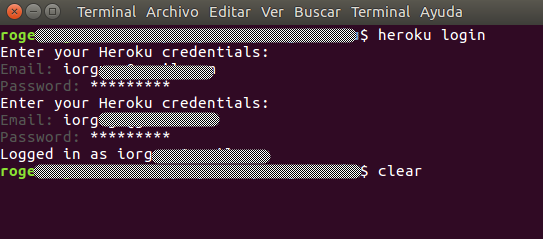
\includegraphics[width=1\textwidth]{../images/heroku_login.png}
    \caption{Login a Heroku.}
    \label{fig:heroku_ssh}
  \end{center}
\end{figure}



\bigskip
Además podemos habilitar una conexión SSH con Heroku de la siguiente manera:


\begin{figure}[!ht]
  \begin{center}
    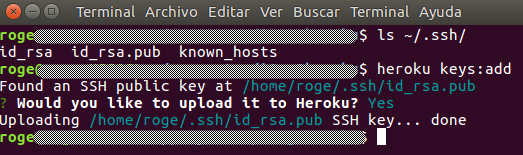
\includegraphics[width=1\textwidth]{../images/heroku_ssh.png}
    \caption{Conexión ssh a Heroku.}
    \label{fig:heroku_ssh}
  \end{center}
\end{figure}


\bigskip
Tras introducir nuestro usuario y contraseña, estamos conectados a Heroku desde nuestra terminal.


\section{Entorno de nuestro código}
Es aquí donde agradeceremos haber utilizado las recomendaciones sobre entornos virtuales y repositorios. Recordemos que nuestros repositorios están separados, en uno el código fuente y en otro el código de nuestra documentación.

\subsection{Entorno virtual}
Tener un entorno virtual bien configurado lo definiríamos como vital en este paso. Tener un entorno desorganizado complicaría mucho las tareas de sincronizar nuestro proyecto con la plataforma Heroku. Las virtudes del entorno virtual son muchas, pero destamos las más importantes que hemos advertido durante el despliegue:

 \begin{itemize}
    \item \textbf{Especificación correcta y única de versiones:}
    
    \bigskip
    En nuestro sistema podremos tener instalada cualquier versión de Django o Python, pero en el entrono  virtual del proyecto sólo tendremos la necesaria. Podemos probar otras versiones del lenguaje o el framework fácilmente creando otro entorno virtual con las versiones deseadas.
    
    \item \textbf{Dependencias bien definidas:}

    \bigskip
    Para desplegar la aplicación deberemos especificar las dependencias a Heroku, tener el entorno virtual con las dependencias mínimas y suficientes para la aplicación es esencial.
    
    \bigskip
    Como nota señalar que, durante el despliegue de Heroku, tuvimos problemas con las dependencias pues, en algún punto del proyecto que no pudimos detectar, todo indica a que instalamos un paquete de forma global desde nuestro entorno virtual. Por esto las dependencias del proyecto aumentaron, pues el entorno necesitaba algunos paquetes generales del sistema operativo. Esto lo descubrimos al subir la aplicación a Heroku y ver que era incapaz de cubrir estas dependencias y fue entonces que decidimos listarlas y descubrimos que no eran correctas.
    
    \bigskip
    Para solucionarlas intentamos desinstalar estas dependencias, pero el sistema parecía no funcionar establemente. Es en este punto cuando vimos la gran virtud de un entorno virtual pues no tuvimos más que crear otro entorno, instalar las dependencias antiguas correctamente y arrancar la aplicación.
    Sin tener un entorno virtual, especificar las dependencias únicas de nuestra aplicación a Heroku hubiese sido prácticamente imposible.
\end{itemize}


\subsection{Repositorio para el proyecto}
  
  Ya estamos conectados a Heroku, nos encontramos en el directorio de nuestro repositorio y dentro de nuestro entorno virtual, ¿cómo subimos nuestro código a Heroku? Aquí es donde Heroku nos pone las cosas sencillas. Con esta plataforma podemos crear un repositorio en el mismo directorio que nuestro repositorio de Git:
  
  \begin{lstlisting}[language=bash]
    $heroku create
    $git push heroku master
  \end{lstlisting}


\subsection{Cambios necesarios para el despliegue}

\bigskip
  Con lo descrito anteriormente ya tenemos subido nuestra aplicación a Heroku pero tendremos nos falta un paso importante a tener en cuenta. Hemos subido un repositorio, con un código fuente, pero Heroku no ejecuta automáticamente el servidor al subirlo, para ello tendremos que añadir un archivo al directorio raíz nombrado \textbf{``Procfile''} y que va a contener un ``dyno''\footnote{Basado en contenedores de Linux, un dyno no es más que un contenedor que ejecuta la instrucción que le indiquemos.} con la instrucción para arrancar el servidor. En nuestro caso: 

  \begin{lstlisting}[language=text]
    web: gunicorn iOrg2.wsgi --log-file -
  \end{lstlisting}

\bigskip
La plataforma ya sabe cómo arrancar el servidor pero no conoce las \textbf{dependencias}. Las dependencias se las especificaremos en un archivo ``requirements.txt''. Para crear este fichero no tenemos más que, dentro de nuestro entorno virtual, ejecutar una orden para listar las dependencias:

\begin{lstlisting}[language=bash]
    $pip freeze requirements.txt
\end{lstlisting}

\bigskip
Nota: en nuestro caso una de las dependencias no era capaz Heroku de satisfacerla, en concreto ``pkg-resources==0.0.0''. Esta dependencia no es necesaria para lanzar el servidor. Para eliminarla cada vez que actualicemos las dependencias hemos creado un pequeño script bash:

\begin{lstlisting}[language=bash]
    #!/bin/bash
    pip freeze | grep -v "pkg-resources" > requirements.txt
\end{lstlisting}


\bigskip
  Algunas configuraciones locales no funcionan en un servidor en línea por lo que habrá que retocarlas a la hora de desplegar el servidor como es el caso de los \textbf{ficheros estáticos} o ``staticfiles'', estos son las hojas de estilos, imágenes cargadas en el html, iconos, etc. Ya que no estábamos familiarizados con estos ficheros al desplegarlos en un servidor, este punto ha dado un poco de trabajo hasta solucionar cómo cargarlos en Heroku. Para ello hemos utilizado el paquete ``WhiteNoise''.

\bigskip
Sólo fue necesario añadir WhiteNoise en los paquetes de Django y habilitar el paquete en el fichero de configuración general: 

\begin{lstlisting}[language=python]
  MIDDLEWARE_CLASSES = [
  'whitenoise.middleware.WhiteNoiseMiddleware',
  ...
  ]    
\end{lstlisting}


\bigskip 
También configuraremos los \textbf{``hosts'' permitidos}, comprobando que no esté únicamente nuestra dirección local y añadiendo la dirección del servidor:

\begin{lstlisting}[language=python]
  ALLOWED_HOSTS = ['localhost','_dirección_del_servidor']
\end{lstlisting}


\bigskip
Ahora sí, tenemos definidas las dependencias, configurados los ficherlos estáticos, permitido el acceso a la nueva dirección y definidas las instrucciones para arrancar el servidor, ya podemos actualizar nuestro repositorio de Heroku y lanzar el servidor indicando a Heroku que ejecute la línea del fichero ``Procfile'':

\begin{lstlisting}[language=bash]
  $ heroku ps:scale web=1
\end{lstlisting}


\bigskip
Ya tenemos nuestra aplicación desplegada en Heroku.

\bigskip
Señalar que podemos lanzar la consola de python desde Heroku si necesitamos realizar cualquier cambio sobre la plataforma, sólo tenemos que ejecutar:


\begin{lstlisting}[language=bash]
  $ heroku run python manage.py shell 
\end{lstlisting}



 \bigskip
 Como podemos ver, para el despliegue de Heroku hemos necesitado realizar algún cambio sobre la configuración local, pero con una correcta gestión del entorno virtual y de los repositorios conseguimos desplegar de forma fácil y eficaz el servidor de testeo.